\refstepcounter{section}
\section*{Lecture 04: Classical Fields}
\addcontentsline{toc}{section}{Lecture 04: Classical Fields}
Let us start with a familiar setting, the spring-mass system in one-dimensions. So, each mass is connected with isotropic springs of natural length $a$ and spring constant $k$, and at some instance, $i^{th}$ spring is displaced from its equilibrium position by an amount $\eta_i$ as shown below:
\begin{figure}[H]
    \centering
    

\tikzset{every picture/.style={line width=0.75pt}} %set default line width to 0.75pt        

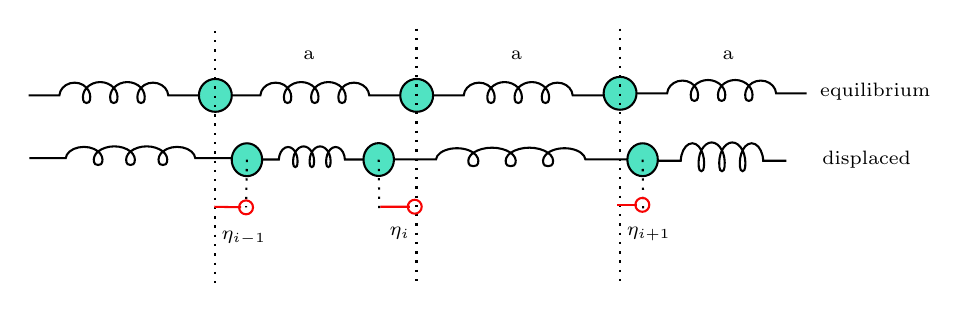
\begin{tikzpicture}[x=0.75pt,y=0.75pt,yscale=-1,xscale=1]
%uncomment if require: \path (0,152); %set diagram left start at 0, and has height of 152

%Shape: Inductor (Air Core) [id:dp4352214065718081] 
\draw   (382,43.64) -- (396.76,43.64) .. controls (396.97,40.93) and (399.02,38.62) .. (401.92,37.81) .. controls (404.82,37) and (407.98,37.86) .. (409.88,39.98) .. controls (411.34,41.63) and (411.94,43.76) .. (411.52,45.84) .. controls (411.52,46.64) and (410.79,47.3) .. (409.88,47.3) .. controls (408.97,47.3) and (408.24,46.64) .. (408.24,45.84) .. controls (407.82,43.76) and (408.42,41.63) .. (409.88,39.98) .. controls (411.58,38.22) and (413.96,37.22) .. (416.44,37.22) .. controls (418.92,37.22) and (421.3,38.22) .. (423,39.98) .. controls (424.46,41.63) and (425.06,43.76) .. (424.64,45.84) .. controls (424.64,46.64) and (423.91,47.3) .. (423,47.3) .. controls (422.09,47.3) and (421.36,46.64) .. (421.36,45.84) .. controls (420.94,43.76) and (421.54,41.63) .. (423,39.98) .. controls (424.7,38.22) and (427.08,37.22) .. (429.56,37.22) .. controls (432.04,37.22) and (434.42,38.22) .. (436.12,39.98) .. controls (437.58,41.63) and (438.18,43.76) .. (437.76,45.84) .. controls (437.76,46.64) and (437.03,47.3) .. (436.12,47.3) .. controls (435.21,47.3) and (434.48,46.64) .. (434.48,45.84) .. controls (434.06,43.76) and (434.66,41.63) .. (436.12,39.98) .. controls (438.02,37.86) and (441.18,37) .. (444.08,37.81) .. controls (446.98,38.62) and (449.03,40.93) .. (449.24,43.64) -- (464,43.64) ;
%Shape: Circle [id:dp6823645192807816] 
\draw  [fill={rgb, 255:red, 80; green, 227; blue, 194 }  ,fill opacity=1 ] (366.16,43.64) .. controls (366.16,39.27) and (369.71,35.72) .. (374.08,35.72) .. controls (378.46,35.72) and (382,39.27) .. (382,43.64) .. controls (382,48.01) and (378.46,51.56) .. (374.08,51.56) .. controls (369.71,51.56) and (366.16,48.01) .. (366.16,43.64) -- cycle ;
%Shape: Inductor (Air Core) [id:dp6724095793711728] 
\draw   (284,44.64) -- (298.76,44.64) .. controls (298.97,41.93) and (301.02,39.62) .. (303.92,38.81) .. controls (306.82,38) and (309.98,38.86) .. (311.88,40.98) .. controls (313.34,42.63) and (313.94,44.76) .. (313.52,46.84) .. controls (313.52,47.64) and (312.79,48.3) .. (311.88,48.3) .. controls (310.97,48.3) and (310.24,47.64) .. (310.24,46.84) .. controls (309.82,44.76) and (310.42,42.63) .. (311.88,40.98) .. controls (313.58,39.22) and (315.96,38.22) .. (318.44,38.22) .. controls (320.92,38.22) and (323.3,39.22) .. (325,40.98) .. controls (326.46,42.63) and (327.06,44.76) .. (326.64,46.84) .. controls (326.64,47.64) and (325.91,48.3) .. (325,48.3) .. controls (324.09,48.3) and (323.36,47.64) .. (323.36,46.84) .. controls (322.94,44.76) and (323.54,42.63) .. (325,40.98) .. controls (326.7,39.22) and (329.08,38.22) .. (331.56,38.22) .. controls (334.04,38.22) and (336.42,39.22) .. (338.12,40.98) .. controls (339.58,42.63) and (340.18,44.76) .. (339.76,46.84) .. controls (339.76,47.64) and (339.03,48.3) .. (338.12,48.3) .. controls (337.21,48.3) and (336.48,47.64) .. (336.48,46.84) .. controls (336.06,44.76) and (336.66,42.63) .. (338.12,40.98) .. controls (340.02,38.86) and (343.18,38) .. (346.08,38.81) .. controls (348.98,39.62) and (351.03,41.93) .. (351.24,44.64) -- (366,44.64) ;
%Shape: Circle [id:dp27398309555614764] 
\draw  [fill={rgb, 255:red, 80; green, 227; blue, 194 }  ,fill opacity=1 ] (268.16,44.64) .. controls (268.16,40.27) and (271.71,36.72) .. (276.08,36.72) .. controls (280.46,36.72) and (284,40.27) .. (284,44.64) .. controls (284,49.01) and (280.46,52.56) .. (276.08,52.56) .. controls (271.71,52.56) and (268.16,49.01) .. (268.16,44.64) -- cycle ;
%Shape: Inductor (Air Core) [id:dp7224489453415708] 
\draw   (186,44.64) -- (200.76,44.64) .. controls (200.97,41.93) and (203.02,39.62) .. (205.92,38.81) .. controls (208.82,38) and (211.98,38.86) .. (213.88,40.98) .. controls (215.34,42.63) and (215.94,44.76) .. (215.52,46.84) .. controls (215.52,47.64) and (214.79,48.3) .. (213.88,48.3) .. controls (212.97,48.3) and (212.24,47.64) .. (212.24,46.84) .. controls (211.82,44.76) and (212.42,42.63) .. (213.88,40.98) .. controls (215.58,39.22) and (217.96,38.22) .. (220.44,38.22) .. controls (222.92,38.22) and (225.3,39.22) .. (227,40.98) .. controls (228.46,42.63) and (229.06,44.76) .. (228.64,46.84) .. controls (228.64,47.64) and (227.91,48.3) .. (227,48.3) .. controls (226.09,48.3) and (225.36,47.64) .. (225.36,46.84) .. controls (224.94,44.76) and (225.54,42.63) .. (227,40.98) .. controls (228.7,39.22) and (231.08,38.22) .. (233.56,38.22) .. controls (236.04,38.22) and (238.42,39.22) .. (240.12,40.98) .. controls (241.58,42.63) and (242.18,44.76) .. (241.76,46.84) .. controls (241.76,47.64) and (241.03,48.3) .. (240.12,48.3) .. controls (239.21,48.3) and (238.48,47.64) .. (238.48,46.84) .. controls (238.06,44.76) and (238.66,42.63) .. (240.12,40.98) .. controls (242.02,38.86) and (245.18,38) .. (248.08,38.81) .. controls (250.98,39.62) and (253.03,41.93) .. (253.24,44.64) -- (268,44.64) ;
%Shape: Circle [id:dp09319907365871849] 
\draw  [fill={rgb, 255:red, 80; green, 227; blue, 194 }  ,fill opacity=1 ] (171.16,44.64) .. controls (171.16,40.27) and (174.71,36.72) .. (179.08,36.72) .. controls (183.46,36.72) and (187,40.27) .. (187,44.64) .. controls (187,49.01) and (183.46,52.56) .. (179.08,52.56) .. controls (174.71,52.56) and (171.16,49.01) .. (171.16,44.64) -- cycle ;
%Shape: Inductor (Air Core) [id:dp13075010063815495] 
\draw   (89.16,44.64) -- (103.92,44.64) .. controls (104.14,41.93) and (106.18,39.62) .. (109.08,38.81) .. controls (111.98,38) and (115.14,38.86) .. (117.04,40.98) .. controls (118.51,42.63) and (119.11,44.76) .. (118.68,46.84) .. controls (118.68,47.64) and (117.95,48.3) .. (117.04,48.3) .. controls (116.14,48.3) and (115.4,47.64) .. (115.4,46.84) .. controls (114.98,44.76) and (115.58,42.63) .. (117.04,40.98) .. controls (118.75,39.22) and (121.12,38.22) .. (123.6,38.22) .. controls (126.09,38.22) and (128.46,39.22) .. (130.16,40.98) .. controls (131.63,42.63) and (132.23,44.76) .. (131.8,46.84) .. controls (131.8,47.64) and (131.07,48.3) .. (130.16,48.3) .. controls (129.26,48.3) and (128.52,47.64) .. (128.52,46.84) .. controls (128.1,44.76) and (128.7,42.63) .. (130.16,40.98) .. controls (131.87,39.22) and (134.24,38.22) .. (136.72,38.22) .. controls (139.21,38.22) and (141.58,39.22) .. (143.28,40.98) .. controls (144.75,42.63) and (145.35,44.76) .. (144.92,46.84) .. controls (144.92,47.64) and (144.19,48.3) .. (143.28,48.3) .. controls (142.38,48.3) and (141.64,47.64) .. (141.64,46.84) .. controls (141.22,44.76) and (141.82,42.63) .. (143.28,40.98) .. controls (145.18,38.86) and (148.34,38) .. (151.24,38.81) .. controls (154.14,39.62) and (156.19,41.93) .. (156.4,44.64) -- (171.16,44.64) ;
%Shape: Inductor (Air Core) [id:dp10489929749363958] 
\draw   (392.12,76.13) -- (403.3,76.13) .. controls (403.46,72.41) and (405.01,69.23) .. (407.2,68.12) .. controls (409.4,67) and (411.79,68.19) .. (413.23,71.1) .. controls (414.34,73.37) and (414.79,76.3) .. (414.47,79.15) .. controls (414.47,80.26) and (413.92,81.17) .. (413.23,81.17) .. controls (412.55,81.17) and (411.99,80.26) .. (411.99,79.15) .. controls (411.67,76.3) and (412.12,73.37) .. (413.23,71.1) .. controls (414.52,68.68) and (416.32,67.31) .. (418.2,67.31) .. controls (420.08,67.31) and (421.88,68.68) .. (423.17,71.1) .. controls (424.28,73.37) and (424.73,76.3) .. (424.41,79.15) .. controls (424.41,80.26) and (423.85,81.17) .. (423.17,81.17) .. controls (422.48,81.17) and (421.93,80.26) .. (421.93,79.15) .. controls (421.61,76.3) and (422.06,73.37) .. (423.17,71.1) .. controls (424.46,68.68) and (426.26,67.31) .. (428.14,67.31) .. controls (430.02,67.31) and (431.81,68.68) .. (433.1,71.1) .. controls (434.21,73.37) and (434.67,76.3) .. (434.35,79.15) .. controls (434.35,80.26) and (433.79,81.17) .. (433.1,81.17) .. controls (432.42,81.17) and (431.86,80.26) .. (431.86,79.15) .. controls (431.54,76.3) and (432,73.37) .. (433.1,71.1) .. controls (434.54,68.19) and (436.94,67) .. (439.13,68.12) .. controls (441.33,69.23) and (442.88,72.41) .. (443.04,76.13) -- (454.22,76.13) ;
%Shape: Ellipse [id:dp979842934415126] 
\draw  [fill={rgb, 255:red, 80; green, 227; blue, 194 }  ,fill opacity=1 ] (377.59,75.64) .. controls (377.59,71.27) and (380.88,67.72) .. (384.93,67.72) .. controls (388.98,67.72) and (392.26,71.27) .. (392.26,75.64) .. controls (392.26,80.01) and (388.98,83.56) .. (384.93,83.56) .. controls (380.88,83.56) and (377.59,80.01) .. (377.59,75.64) -- cycle ;
%Shape: Ellipse [id:dp1206931681241672] 
\draw  [fill={rgb, 255:red, 80; green, 227; blue, 194 }  ,fill opacity=1 ] (250.45,75.55) .. controls (250.45,71.18) and (253.73,67.64) .. (257.78,67.64) .. controls (261.84,67.64) and (265.12,71.18) .. (265.12,75.55) .. controls (265.12,79.93) and (261.84,83.47) .. (257.78,83.47) .. controls (253.73,83.47) and (250.45,79.93) .. (250.45,75.55) -- cycle ;
%Shape: Inductor (Air Core) [id:dp6543203659259691] 
\draw   (200.7,75.55) -- (209.66,75.55) .. controls (209.79,72.88) and (211.03,70.6) .. (212.79,69.8) .. controls (214.55,69) and (216.46,69.85) .. (217.62,71.94) .. controls (218.5,73.57) and (218.87,75.68) .. (218.61,77.72) .. controls (218.61,78.52) and (218.17,79.17) .. (217.62,79.17) .. controls (217.07,79.17) and (216.62,78.52) .. (216.62,77.72) .. controls (216.36,75.68) and (216.73,73.57) .. (217.62,71.94) .. controls (218.65,70.21) and (220.09,69.22) .. (221.6,69.22) .. controls (223.1,69.22) and (224.54,70.21) .. (225.58,71.94) .. controls (226.46,73.57) and (226.83,75.68) .. (226.57,77.72) .. controls (226.57,78.52) and (226.12,79.17) .. (225.58,79.17) .. controls (225.03,79.17) and (224.58,78.52) .. (224.58,77.72) .. controls (224.32,75.68) and (224.69,73.57) .. (225.58,71.94) .. controls (226.61,70.21) and (228.05,69.22) .. (229.56,69.22) .. controls (231.06,69.22) and (232.5,70.21) .. (233.54,71.94) .. controls (234.42,73.57) and (234.79,75.68) .. (234.53,77.72) .. controls (234.53,78.52) and (234.08,79.17) .. (233.54,79.17) .. controls (232.99,79.17) and (232.54,78.52) .. (232.54,77.72) .. controls (232.28,75.68) and (232.65,73.57) .. (233.54,71.94) .. controls (234.69,69.85) and (236.61,69) .. (238.36,69.8) .. controls (240.12,70.6) and (241.37,72.88) .. (241.5,75.55) -- (250.45,75.55) ;
%Shape: Ellipse [id:dp10858887431639541] 
\draw  [fill={rgb, 255:red, 80; green, 227; blue, 194 }  ,fill opacity=1 ] (186.96,75.64) .. controls (186.96,71.27) and (190.24,67.72) .. (194.29,67.72) .. controls (198.34,67.72) and (201.63,71.27) .. (201.63,75.64) .. controls (201.63,80.01) and (198.34,83.56) .. (194.29,83.56) .. controls (190.24,83.56) and (186.96,80.01) .. (186.96,75.64) -- cycle ;
%Shape: Inductor (Air Core) [id:dp3912229968736276] 
\draw   (89.45,74.91) -- (107,74.91) .. controls (107.25,72.5) and (109.69,70.44) .. (113.14,69.72) .. controls (116.59,69) and (120.34,69.77) .. (122.6,71.65) .. controls (124.34,73.12) and (125.06,75.02) .. (124.55,76.86) .. controls (124.55,77.58) and (123.68,78.17) .. (122.6,78.17) .. controls (121.53,78.17) and (120.65,77.58) .. (120.65,76.86) .. controls (120.15,75.02) and (120.86,73.12) .. (122.6,71.65) .. controls (124.63,70.09) and (127.45,69.2) .. (130.4,69.2) .. controls (133.36,69.2) and (136.18,70.09) .. (138.2,71.65) .. controls (139.95,73.12) and (140.66,75.02) .. (140.15,76.86) .. controls (140.15,77.58) and (139.28,78.17) .. (138.2,78.17) .. controls (137.13,78.17) and (136.25,77.58) .. (136.25,76.86) .. controls (135.75,75.02) and (136.46,73.12) .. (138.2,71.65) .. controls (140.23,70.09) and (143.05,69.2) .. (146.01,69.2) .. controls (148.96,69.2) and (151.78,70.09) .. (153.81,71.65) .. controls (155.55,73.12) and (156.26,75.02) .. (155.76,76.86) .. controls (155.76,77.58) and (154.88,78.17) .. (153.81,78.17) .. controls (152.73,78.17) and (151.86,77.58) .. (151.86,76.86) .. controls (151.35,75.02) and (152.06,73.12) .. (153.81,71.65) .. controls (156.07,69.77) and (159.82,69) .. (163.27,69.72) .. controls (166.72,70.44) and (169.15,72.5) .. (169.41,74.91) -- (186.96,74.91) ;
%Straight Lines [id:da24228885261380384] 
\draw  [dash pattern={on 0.84pt off 2.51pt}]  (179,13.52) -- (179,138.52) ;
%Straight Lines [id:da8719944335955531] 
\draw  [dash pattern={on 0.84pt off 2.51pt}]  (276,12.52) -- (276,137.52) ;
%Straight Lines [id:da2861301148607793] 
\draw  [dash pattern={on 0.84pt off 2.51pt}]  (374,12.52) -- (374,137.52) ;
%Shape: Inductor (Air Core) [id:dp6617281157596067] 
\draw   (265.12,75.51) -- (285.37,75.51) .. controls (285.66,73.12) and (288.47,71.08) .. (292.45,70.36) .. controls (296.43,69.65) and (300.77,70.41) .. (303.37,72.28) .. controls (305.38,73.74) and (306.2,75.62) .. (305.62,77.46) .. controls (305.62,78.17) and (304.62,78.75) .. (303.37,78.75) .. controls (302.13,78.75) and (301.12,78.17) .. (301.12,77.46) .. controls (300.54,75.62) and (301.36,73.74) .. (303.37,72.28) .. controls (305.71,70.72) and (308.97,69.84) .. (312.38,69.84) .. controls (315.78,69.84) and (319.04,70.72) .. (321.38,72.28) .. controls (323.39,73.74) and (324.21,75.62) .. (323.63,77.46) .. controls (323.63,78.17) and (322.62,78.75) .. (321.38,78.75) .. controls (320.13,78.75) and (319.13,78.17) .. (319.13,77.46) .. controls (318.55,75.62) and (319.37,73.74) .. (321.38,72.28) .. controls (323.71,70.72) and (326.97,69.84) .. (330.38,69.84) .. controls (333.78,69.84) and (337.04,70.72) .. (339.38,72.28) .. controls (341.39,73.74) and (342.21,75.62) .. (341.63,77.46) .. controls (341.63,78.17) and (340.62,78.75) .. (339.38,78.75) .. controls (338.14,78.75) and (337.13,78.17) .. (337.13,77.46) .. controls (336.55,75.62) and (337.37,73.74) .. (339.38,72.28) .. controls (341.99,70.41) and (346.32,69.65) .. (350.3,70.36) .. controls (354.28,71.08) and (357.09,73.12) .. (357.38,75.51) -- (377.63,75.51) ;
%Straight Lines [id:da36773613103153313] 
\draw  [dash pattern={on 0.84pt off 2.51pt}]  (194.29,75.64) -- (193.88,98.59) ;
%Straight Lines [id:da5894276902305823] 
\draw  [dash pattern={on 0.84pt off 2.51pt}]  (257.78,75.55) -- (258.07,99.68) ;
%Straight Lines [id:da01583668385191661] 
\draw  [dash pattern={on 0.84pt off 2.51pt}]  (384.93,75.64) -- (385.22,99.77) ;
%Straight Lines [id:da627974370607899] 
\draw [color={rgb, 255:red, 247; green, 4; blue, 4 }  ,draw opacity=1 ]   (178.56,98.31) -- (191.53,98.55) ;
\draw [shift={(193.88,98.59)}, rotate = 1.06] [color={rgb, 255:red, 247; green, 4; blue, 4 }  ,draw opacity=1 ][line width=0.75]      (0, 0) circle [x radius= 3.35, y radius= 3.35]   ;
%Straight Lines [id:da2390864919900585] 
\draw [color={rgb, 255:red, 247; green, 4; blue, 4 }  ,draw opacity=1 ]   (258.56,98.31) -- (272.8,98.29) ;
\draw [shift={(275.15,98.28)}, rotate = 359.92] [color={rgb, 255:red, 247; green, 4; blue, 4 }  ,draw opacity=1 ][line width=0.75]      (0, 0) circle [x radius= 3.35, y radius= 3.35]   ;
%Straight Lines [id:da06742391213277577] 
\draw [color={rgb, 255:red, 247; green, 4; blue, 4 }  ,draw opacity=1 ]   (372.8,97.38) -- (382.45,97.38) ;
\draw [shift={(384.8,97.38)}, rotate = 0] [color={rgb, 255:red, 247; green, 4; blue, 4 }  ,draw opacity=1 ][line width=0.75]      (0, 0) circle [x radius= 3.35, y radius= 3.35]   ;

% Text Node
\draw (180.56,108.71) node [anchor=north west][inner sep=0.75pt]  [font=\scriptsize]  {$\eta _{i-1}$};
% Text Node
\draw (261.56,106.71) node [anchor=north west][inner sep=0.75pt]  [font=\scriptsize]  {$\eta _{i}$};
% Text Node
\draw (375.8,106.78) node [anchor=north west][inner sep=0.75pt]  [font=\scriptsize]  {$\eta _{i+1}$};
% Text Node
\draw (220,22) node [anchor=north west][inner sep=0.75pt]  [font=\scriptsize] [align=left] {a};
% Text Node
\draw (320,22) node [anchor=north west][inner sep=0.75pt]  [font=\scriptsize] [align=left] {a};
% Text Node
\draw (422,22) node [anchor=north west][inner sep=0.75pt]  [font=\scriptsize] [align=left] {a};
% Text Node
\draw (470,70) node [anchor=north west][inner sep=0.75pt]  [font=\scriptsize] [align=left] {displaced};
% Text Node
\draw (469,37) node [anchor=north west][inner sep=0.75pt]  [font=\scriptsize] [align=left] {equilibrium};


\end{tikzpicture}

    \caption{A spring-mass system; each mass is displaced by some amount from its equilibrium position}
\end{figure}
Then the kinetic and potential energies can be written as:
$$T = \frac{1}{2}\sum\limits_i\dot{\eta}_i^2 \qquad \quad V = \frac{1}{2}\sum\limits_{i}k \qty(\eta_{i+}-\eta_i)^2 $$
From this, the Langrangian of the system is obtained as:
$$L = T-V = \frac{1}{2}\sum \limits_i a \qty[\qty(\sfrac{m}{a}) \dot{\eta}_i^2 - ka \qty(\frac{\eta_{i+1}-\eta_i}{a})^2] = a\sum\limits_i L_i $$
The resulting ELEOM are:
$$\dv{t}\qty(\pdv{L}{\dot{\eta}_i}) = \pdv{L}{\eta}\implies \qty(\sfrac{m}{a})\ddot{\eta}_i - ka \qty(\frac{\eta_{i+1}-\eta_i}{a^2}) + ka\qty(\frac{\eta_i - \eta_{i-1}}{a^2})=0$$
In the \textit{continuum} limit, that is, $a\rightarrow 0$ (so, the system kind of becomes like a rod), we have:
\begin{align*}
    \frac{m}{a} &\;\longrightarrow\; \mu 
        && :\text{mass per unit length of the rod} \\[6pt]
    ka &\;\longrightarrow\; Y 
        && :\text{Young's modulus of the rod} \\[6pt]
    i &\;\longrightarrow\; x 
        && :\text{position label} \\[6pt]
    \eta_i &\;\longrightarrow\; \eta(x) 
        && :\text{field} \\[6pt]
    \frac{\eta_{i+1}-\eta_{i}}{a} &\;\longrightarrow\; \frac{d\eta}{dx} 
        && :\text{derivative} \\[6pt]
    \sum_{i} &\;\longrightarrow\; \int dx 
        && :\text{integral}
\end{align*}
Hence in the continuum limits, the ELEOM becomes:
\begin{align*}
    \lim\limits_{a\rightarrow 0} \qty(\mu \dv[2]{\eta}{t} - \frac{Y}{a} \dv{\eta}{x}\Bigg|_{x} + \frac{Y}{a}\dv{\eta}{x}\Bigg|_{x-a}) = 0 \implies \mu \dv[2]{\eta}{t}  - Y \dv[2]{\eta}{x} = 0
\end{align*}
Defining the velocity as $v:= \sqrt{\frac{Y}{\mu}}$, we obtain the wave-equation:
$$\frac{1}{v^2}\dv[2]{\eta}{t} -\dv[2]{\eta}{x} = 0 $$
Note that, in this case, position becomes a mere label like in the discrete case, $i$ just labelled the index of the $i^{\mathrm{th}}$ mass. Also, technically, $\eta$ can also depend on time, so it is better to write it as $\eta(x,t)$. \\[0.2cm]
Position and time, both are kind of labels and thus are independent. Hence, total and partial derivatives coincide in this case. Note that in continuum, the Langrangian itself becomes an integral of the form:
$$L = \frac{1}{2}\int \qty[\mu \dot{\eta}^2 - Y \qty(\dv{\eta}{x})^2] dx$$
The bracketted term is the Lagrangian density, denoted by $\SL$ and hence, the Lagrangian is the space integral of the Langrangian density: $$L = \int \SL \ dx$$
Henceforth, we allow ourselves to be \textit{sloppy} enough and refer to Lagrangian density as simply the Langrangian when context is clear.
\subsection{Action tells a lot!}
Let us now consider a general setting. So, the Lagrangian density can be a function of the field, the spatial and temporal derivatives and space and time themselves. In compact notation, we write:
$$\SL \equiv \SL(\phi, \partial_\mu \phi, x^\mu)$$
Remember, that we define the classical action $S$ as:
$$S = \int\limits_{t_1}^{t_2} dt \ L = \int\limits_{t_1}^{t_2} dt \int d^3\vb{x}\ \SL(\phi, \partial_\mu \phi, x^\mu) = \int d^4\vb{x} \ \SL(\phi, \partial_\mu \phi, x^\mu)$$
The integration is now over space-time. We now want to use Hamilton's principle, which states that, under fixed boundary conditions, the system takes a path in configuration space for which the action is stationary, that is, 
$$\delta S =0$$
Note that action is a linear-functional which takes a field $\phi$ as input and returns a real number\footnote{For functionals, a common notation for the input is to use square brackets, that is, if $A$ is a linear functional taking function $f$ as input, $A[f]\in \re$}. Let us consider a variation in the field itself: $\phi \longrightarrow \ \phi' = \phi + \delta \phi$ such that $\delta\phi$ vanishes at the boundary of the integration domain.
Then we have the following:
$$\delta S = S[\phi'] - S[\phi] = \int d^4\vb{x}\ \qty(\SL(\phi', \partial_\mu \phi', x^\mu) -\SL(\phi, \partial_\mu \phi, x^\mu) )$$
Now, we try to find what the above quantity is:
\begin{align*}
    \SL(\phi', \partial_\mu \phi', x^\mu) &= \SL(\phi+\delta\phi, \partial_\mu (\phi+\delta \phi), x^\mu)\\
&=L(\phi, \partial_\mu \phi, x^\mu) + \pdv{\SL}{\phi}\delta\phi + \pdv{\SL}{(\partial_\mu\phi)}\delta(\partial_\mu\phi)
\end{align*}
Also note that $\delta(\partial_\mu\phi) = \partial_\mu(\delta\phi)$. Hence, from the above expression, we obtain that:
$$\delta S = \int d^4\vb{x}\ \qty(\pdv{\SL}{\phi}\delta\phi + \pdv{\SL}{(\partial_\mu\phi)}\partial_\mu(\delta\phi))$$
Using \textit{integration by parts} on the second term, we obtain:
$$\int d^4\vb{x}\ \pdv{\SL}{(\partial_\mu\phi)}\partial_\mu(\delta\phi) = -\int d^4\vb{x}\ \partial_\mu\qty(\pdv{\SL}{(\partial_\mu\phi)})\delta\phi + \qty(\pdv{\SL}{(\partial_\mu\phi)}\delta\phi)\Biggr|_{\mathrm{boundary}}$$
The variation in the field vanishes at the boundary by our assumption. Then we obtain, for the variation of the action:
$$\delta S =\int d^4\vb{x}\ \qty(\pdv{\SL}{\phi} - \partial_\mu\qty(\pdv{\SL}{(\partial_\mu\phi)}))\delta\phi=0 $$
Since the variation in the field was arbitrary, we obtain the Lagrange's equations for the field as:
$$\pdv{\SL}{\phi} - \partial_\mu\qty(\pdv{\SL}{(\partial_\mu\phi)})=0$$
In general, we want the action to be \textit{Lorentz} invariant, in order to maintain the universality of physical laws. Since the volume element of Minkowski space $d^4\vb{x}$ is invariant under Lorentz transformations, this imply that $\SL$ should also be constructed of Lorentz-invariant quantities.\\[0.2cm] The field $\phi$ (and all its powers) is a Lorentz \textit{scalar} and is hence invariant. The derivative $\partial_\mu \phi$ is not invariant, however, $\partial^\mu\partial_\mu \phi$ is. Bilinears like $(\partial^\mu\phi)(\partial_\mu\phi)$ are also invariant. Hence, a simple Lagrangian should be constructed of these quantities. Let us consider the Lagrangian:
$$\SL = \frac{1}{2}(\partial^\mu\phi)(\partial_\mu\phi) - \frac{1}{2}m^2\phi^2 = \frac{1}{2}\eta^{\mu\nu}(\partial_\nu \phi) (\partial_\mu\phi)-\frac{1}{2}m^2\phi^2$$
Then, from the Lagrange's equations,
\begin{align*}
    \pdv{\SL}{\phi} &= -m^2\phi \\
    \pdv{\SL}{(\partial_\mu \phi)} &= \frac{1}{2} \eta^{\mu\nu} \qty(\partial_\nu \phi +\partial_\mu\phi \tensor{\delta}{^\mu _\nu})\\
    &=\frac{1}{2} \eta^{\mu\nu} (2\times \partial_\nu \phi)\\
    &=\eta^{\mu\nu}\partial_\nu \phi\\
    &=\partial^\mu\phi
\end{align*}
Then we finally obtain:
$$-m^2\phi - \partial_\mu\partial^\mu\phi=0 \implies (\partial_\mu\partial^\mu+m^2)\phi = 0$$
This is the KG equation that we had seen earlier. Thus, the above Lagrangian models the KG equation.
